Cluster \textbf{Controller} is the fundamental cluster in \emph{Flat Hunt}. Here are the classes that ``control'' the actions. They make sure that the displayer classes in cluster \textbf{View} display the proper information, which they get from the \textbf{Model} classes. For example, feature \textit{prepare} in class \texttt{MAIN\_CONTROLLER} controls the display update by calling \textit{game\_scene.center\_on\_player (game.current\_player)}.

\begin{itemize}
  \item{\textbf{MAIN\_CONTROLLER}: The \texttt{MAIN\_CONTROLLER} is (as the name suggests) responsible for many things. It provides access to the \texttt{GAME\_SCENE}, to class \texttt{GAME} and to the whole \emph{TRAFFIC} library, which is responsible for the visualization of the map.}
  \item{\textbf{GAME}: Class \texttt{GAME} features the game logic. It knows which player's turn it is, and also, since it is an heir of \texttt{GAME\_CONSTANTS}, what state the game is in.}
\end{itemize}

\begin{figure}[h]
\centerline{\hbox{  
  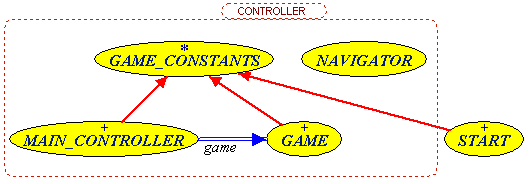
\includegraphics[width=135mm]{controller}
  }}
\caption{Diagram of the Controller Cluster}
\label{controllerdiagram}
\end{figure}
